% -----------------------------------------------------------------
% 3. Cronograma: Gantt, Red y Compresión
% -----------------------------------------------------------------
\section{Cronograma del Proyecto}

\subsection{Diagrama de Gantt}

% Requiere en el preámbulo: \usepackage{pgfgantt} \usepackage{float}
\begin{figure}[H]
\centering
\begin{ganttchart}[
    % --- tamaño y grillas ---
    expand chart=\textwidth,      % ocupa todo el ancho útil
    hgrid, vgrid,
    y unit chart=0.6cm,
    bar height=0.5,
    milestone height=0.6,
    % --- colores / estilos (usa EAFIT-blue definido en Settings) ---
    title/.append style       ={fill=EAFIT-blue!12, draw=EAFIT-blue!40},
    title label font          =\bfseries\footnotesize,
    bar/.append style         ={fill=EAFIT-blue!25, draw=EAFIT-blue!70},
    bar label font            =\scriptsize,
    group/.append style       ={fill=EAFIT-blue!15, draw=EAFIT-blue!70},
    milestone/.append style   ={fill=red!70, draw=red!80!black},
    link/.style               ={-latex, draw=EAFIT-blue!80},
]{1}{27}
\gantttitle{Cronograma (unidades de tiempo)}{27} \\
\gantttitlelist{1,...,27}{1} \\

% Barras (start = ES ; end = EF) ya calculadas con lags/leads incorporados
\ganttbar[name=A]{A}{1}{1} \\
\ganttbar[name=B]{B}{2}{4} \\
\ganttbar[name=C]{C}{2}{5} \\
\ganttbar[name=D]{D}{2}{3} \\
\ganttbar[name=E]{E}{5}{9} \\
\ganttbar[name=M]{M}{4}{8} \\
\ganttbar[name=F]{F}{10}{12} \\
\ganttbar[name=N]{N}{9}{11} \\
\ganttbar[name=O]{O}{6}{9} \\
\ganttbar[name=G]{G}{13}{14} \\
\ganttbar[name=H]{H}{13}{16} \\
\ganttbar[name=P]{P}{11}{15} \\
\ganttbar[name=T]{T}{10}{15} \\
\ganttbar[name=I]{I}{15}{17} \\
\ganttbar[name=K]{K}{17}{20} \\
\ganttbar[name=Q]{Q}{16}{18} \\
\ganttbar[name=J]{J}{18}{19} \\
\ganttbar[name=R]{R}{19}{20} \\
\ganttbar[name=S]{S}{17}{20} \\
\ganttbar[name=L]{L}{22}{22} \\
\ganttbar[name=W]{W}{20}{20} \\
\ganttbar[name=V]{V}{21}{22} \\
\ganttbar[name=U]{U}{22}{26} \\
\ganttbar[name=X]{X}{23}{25} \\
\ganttbar[name=Y]{Y}{26}{27} \\
\ganttmilestone[name=Z]{Z}{27}

% --- Vínculos (flechas). Nota: los leads/lags ya están reflejados en fechas.
% Origen
\ganttlink{A}{B}   % A -> B
\ganttlink{A}{C}   % A -> C
\ganttlink{A}{D}   % A -> D

% Rama B-E-F
\ganttlink{B}{E}   % B -> E
\ganttlink{E}{F}   % E -> F

% G con dos predecesoras (F; C con lag C+6 ya reflejado en fechas)
\ganttlink{F}{G}   % F -> G
\ganttlink{C}{G}   % C -> G

% H y K
\ganttlink{F}{H}   % F -> H
\ganttlink{H}{K}   % H -> K

% I-J-W
\ganttlink{G}{I}   % G -> I
\ganttlink{I}{J}   % I -> J
\ganttlink{J}{W}   % J -> W

% L con dos predecesoras (K; J con lag J+2 ya reflejado)
\ganttlink{J}{L}   % J -> L
\ganttlink{K}{L}   % K -> L

% M-N-O-T rama desde D (O con lead -3 respecto a M ya reflejado)
\ganttlink{D}{M}   % D -> M
\ganttlink{M}{N}   % M -> N
\ganttlink{M}{O}   % M -> O
\ganttlink{O}{T}   % O -> T

% P-Q-R-S-V
\ganttlink{N}{P}   % N -> P (lead -1 ya reflejado)
\ganttlink{P}{Q}   % P -> Q
\ganttlink{Q}{R}   % Q -> R
\ganttlink{Q}{S}   % Q -> S (lead -2 ya reflejado)
\ganttlink{R}{V}   % Q -> R -> V

% U con dos predecesoras (S; T con T+6 ya reflejado)
\ganttlink{S}{U}   % S -> U
\ganttlink{T}{U}   % T -> U

% X con dos predecesoras (W; V)
\ganttlink{V}{X}   % V -> X
\ganttlink{W}{X}   % W -> X

% Y con dos predecesoras (L; X con lag L+2 ya reflejado)
\ganttlink{X}{Y}   % X -> Y
\ganttlink{L}{Y}   % L -> Y

% Cierre
\ganttlink{Y}{Z}   % Y -> Z
\ganttlink{U}{Z}   % U -> Z

\end{ganttchart}
\caption{Diagrama de Gantt del proyecto (duración total = 27 unidades). Los vínculos ilustran precedencias; los \emph{leads/lags} están incorporados en las fechas de inicio/fin de cada barra.}
\label{fig:gantt}
\end{figure}

\subsection{Diagrama de Red}

El diagrama de red (red de precedencias) incluye inicios y finales tempranos/tardíos, holguras libres y totales, y rutas críticas.

\begin{figure}[H]
  \centering
  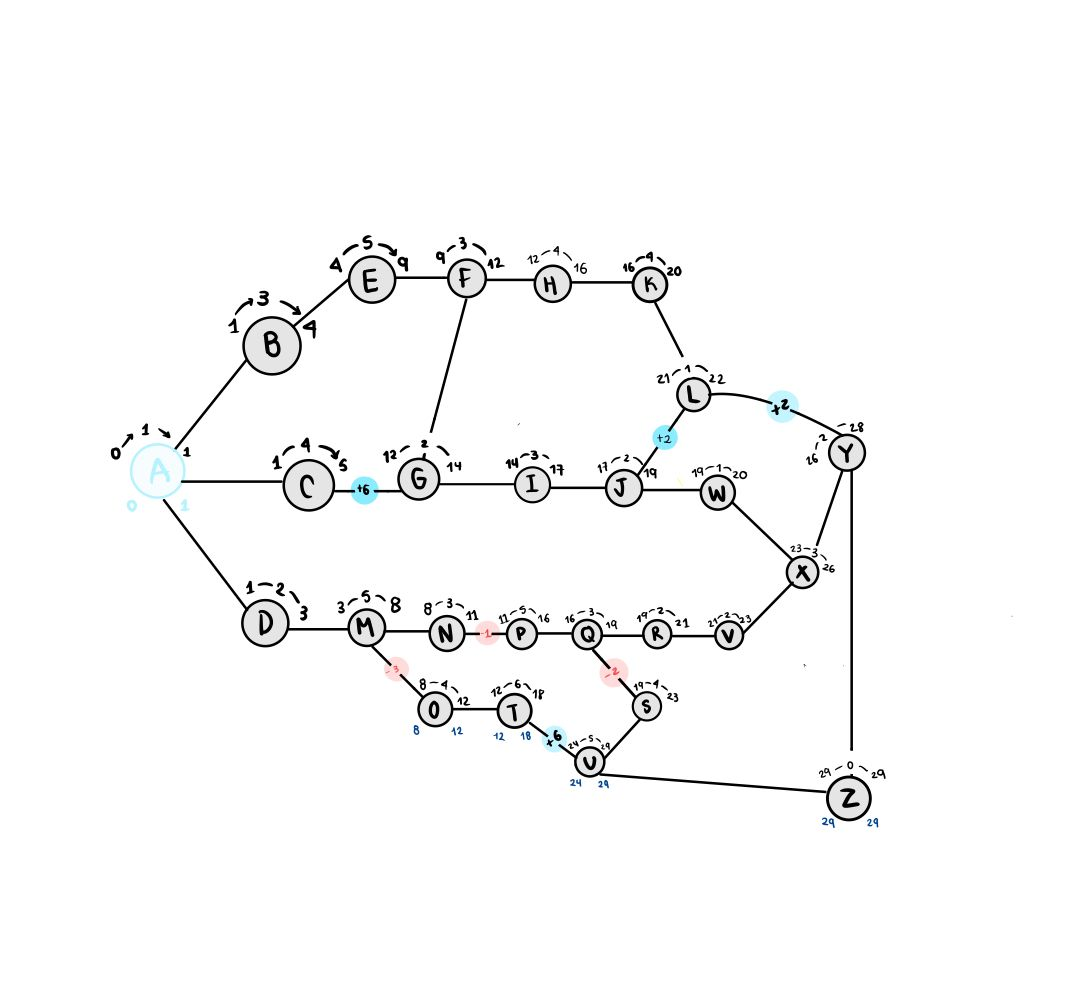
\includegraphics[width=0.8\textwidth]{Figures/0. General/network_diagram.jpeg}
  \caption{Diagrama de red con actividades, holguras y ruta crítica.}
  \label{fig:red}
\end{figure}

\subsection{Compresión del Cronograma: técnicas y escenarios}

\subsubsection*{Técnicas principales}

Según el \emph{PMBOK Guide} \cite{PMBOK}, existen dos técnicas centrales de compresión de cronograma:

\begin{itemize}
    \item \textbf{Fast-tracking (solapamiento lógico):} consiste en ejecutar actividades en paralelo modificando relaciones (FS $\rightarrow$ SS) o introduciendo \emph{leads} (adelantos). Permite reducir tiempo pero aumenta la probabilidad de retrabajo y riesgos de coordinación.
    \item \textbf{Crashing (aceleración con recursos):} consiste en reducir la duración de actividades en la(s) ruta(s) crítica(s) agregando recursos adicionales, turnos extendidos o tecnologías más rápidas. Implica un costo adicional, medido con la pendiente de crash: 
    \[
      \frac{C_{crash}-C_{normal}}{T_{normal}-T_{crash}}
    \]
    \cite{Kerzner2017}.
\end{itemize}

\subsubsection*{Ruta crítica base y duración}

Con las dependencias y posposiciones dadas, la duración total del proyecto es \textbf{27} unidades.  
Una ruta crítica representativa es:
\[
A \rightarrow D \rightarrow M \rightarrow N \rightarrow P \rightarrow Q \rightarrow R \rightarrow V \rightarrow X \rightarrow Y \rightarrow Z.
\]
Comprimir actividades fuera de esta ruta no reduce la fecha final.

\subsubsection*{Escenario 1: \emph{Crashing} selectivo}

En este escenario se busca intervenir actividades con alto impacto en la ruta crítica:

\begin{itemize}
    \item Reducir \textbf{P} de 5 a 3 unidades mediante más cuadrillas de trabajo.
    \item Reducir \textbf{X} de 3 a 2 unidades con más personal/equipo.
    \item Reducir \textbf{T} de 6 a 5 unidades, evitando que la rama \(U\) se acerque al camino crítico.
\end{itemize}

\textbf{Resultado:} duración de \textbf{26} unidades. El hito \(Y\) sigue gobernando el final del proyecto, pero \(U\) queda con un colchón de 1 unidad.  
\textbf{Riesgos:} incremento de costos por recursos adicionales y sobrecarga en la gestión de personal.

\subsubsection*{Escenario 2: combinación de \emph{Fast-tracking} + \emph{Crashing}}

En este escenario se aplican ambas técnicas para lograr una reducción mayor:

\begin{itemize}
    \item Aumentar el \emph{lead} en la relación \(N \rightarrow P\) a \(-3\), iniciando \(P\) antes de finalizar \(N\).
    \item Cambiar la relación \(Q \rightarrow R\) a \textbf{SS+1}.
    \item Reducir \textbf{X} de 3 a 1 unidad (\emph{crashing}).
    \item Eliminar el retraso \((J{+}2)\) en \(L \rightarrow Y\).
    \item Reducir \textbf{T} de 6 a 5 unidades.
\end{itemize}

\textbf{Resultado:} duración aproximada de \textbf{25} unidades.  
\textbf{Riesgos:} mayor complejidad en la coordinación, riesgo de inconsistencias y sobrecarga en la integración de entregables.  
Se recomienda mitigar estos riesgos con \emph{checkpoints} semanales, controles de calidad intermedios y un plan de gestión de cambios \cite{PMBOK,Kerzner2017}.

